\documentclass{beamer}
% beamer is 128x96 mm
\usepackage{pgf,tikz}
\usepackage{import}
\usepackage{subfig}
\usepackage{float}
\usepackage{xmpmulti}
\usepackage{hyperref}
\usepackage{natbib}

\usetikzlibrary{arrows}

\title{Projector Keystone Correction using FPGA }
\author{Ganesh Ajjanagadde \and Shantanu Jain \and James Thomas}
\date{\today}

\begin{document}
\maketitle

\begin{frame}
\frametitle{Background}
\begin{itemize}
\item Portable projectors are everywhere today!
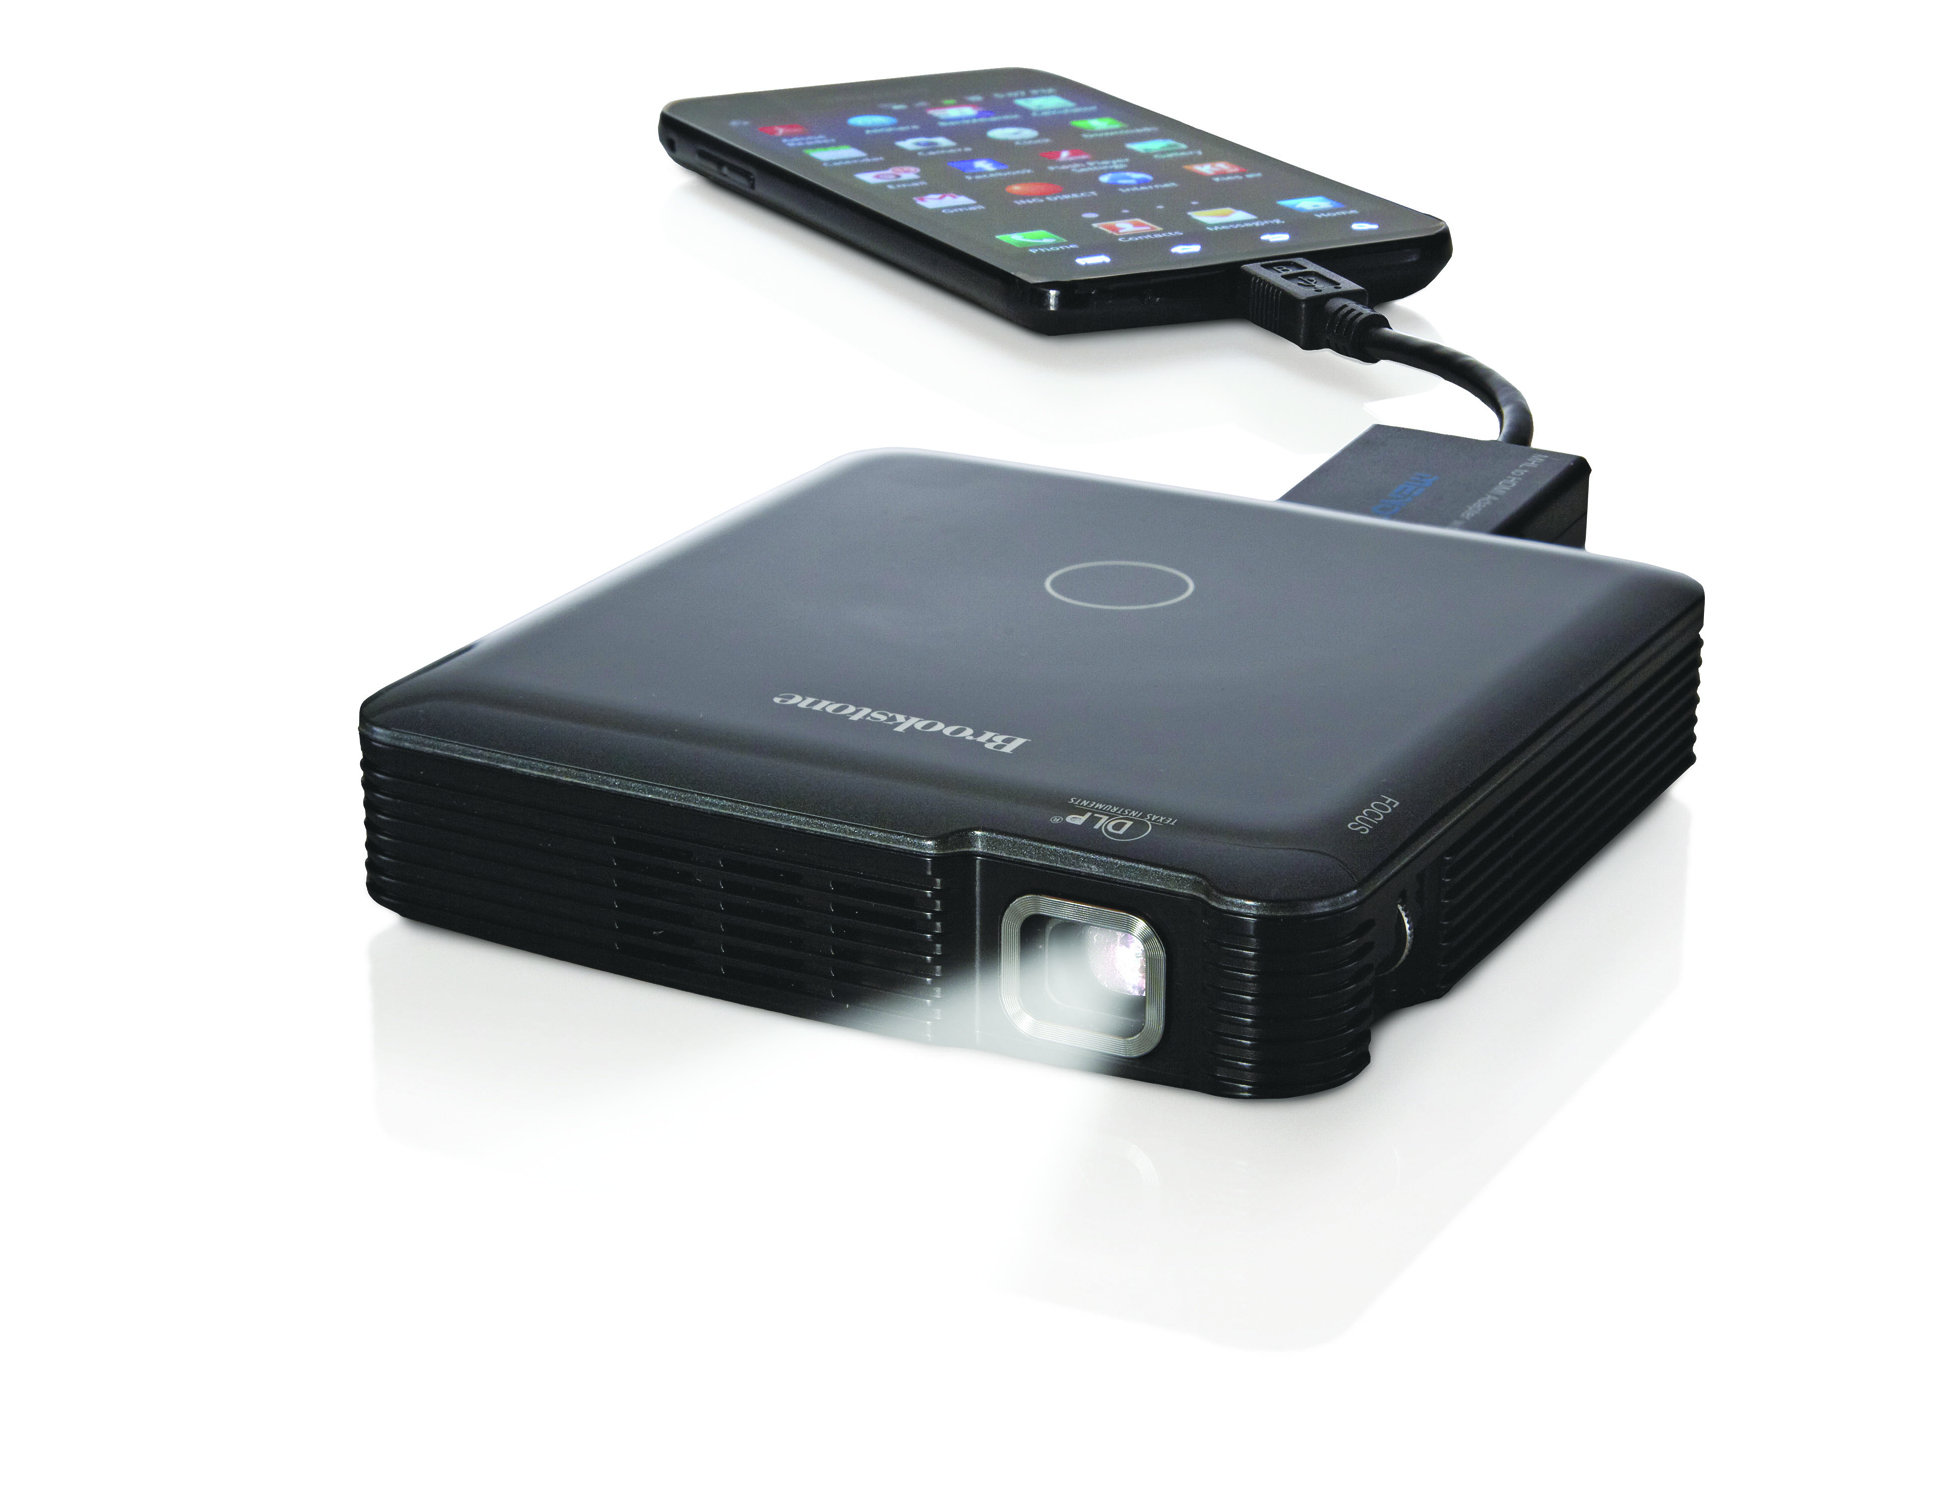
\includegraphics[height=0.6\textheight]{./img/digital_projector}
\item What's the catch?
\pause
\item They are often tricky to setup due to the keystone effect
\end{itemize}
\end{frame}

\begin{frame}
\frametitle{Keystone Effect}
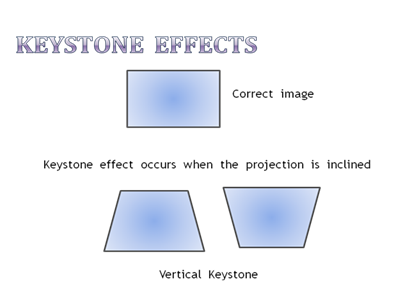
\includegraphics[height=0.8\textheight]{./img/keystone_effect}
\end{frame}

\begin{frame}
\frametitle{Previous Work}
\begin{itemize}
\item \citet{raskar2001self}
\item \citet{sukthankar2001smarter}
\item Both of these use complex software algorithms
\pause
\item Our contribution is creating a simple, FPGA prototype
\end{itemize}
\end{frame}

\begin{frame}
\frametitle{Block Diagram}
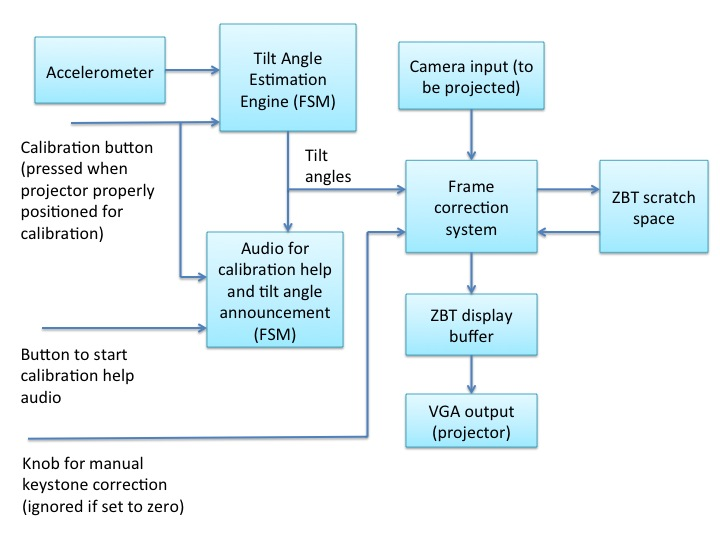
\includegraphics[width=\textwidth]{./img/block_diag}
\end{frame}

\begin{frame}
\frametitle{The Physics of a Projector}
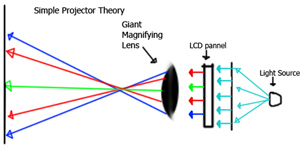
\includegraphics[height=0.5\textheight]{./img/projector_physics}
\end{frame}

\begin{frame}
\frametitle{A Mathematical Model}
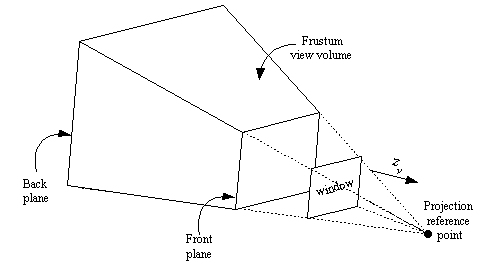
\includegraphics[height=0.5\textheight]{./img/projective_frustrum}
\end{frame}

\begin{frame}
\frametitle{Projective Transformation}
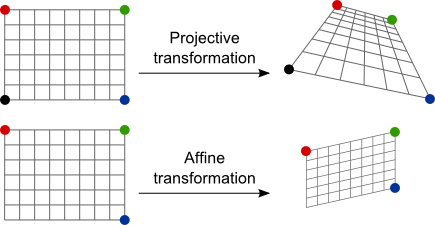
\includegraphics[height=0.5\textheight]{./img/projective_transform}
\end{frame}

\begin{frame}
\frametitle{The Projection Equation}
\begin{itemize}
\item Let $(x, y)$ denote the source image coordinates
\item Let $(X, Y)$ denote the coordinates on the screen
\item $(X, Y)$ = $\left( \frac{p_1x + p_2y + 1}{p_3x + p_4y + 1}, \frac{p_5x + p_6y + 1}{p_7x + p_8y + 1} \right)$
\item Coefficients depend on the tilt of the projector through trigonometry
\pause
\item By projecting a known image, we have 8 equations in 8 unknowns
\item Will require implementing a full-fledged Gaussian elimination routine on the FPGA
\item Too hard, will be final (unlikely) stretch goal
\item How can we simplify?
\end{itemize}
\end{frame}

\begin{frame}
\frametitle{The Simplification}
\begin{itemize}
\item Focus on the 2 axes of interest, and compute inverse mapping
\item Vertical direction is relatively easy
\item Side-to-side direction is harder
\pause
\item Have to compute maximum rectangle of correct aspect ratio
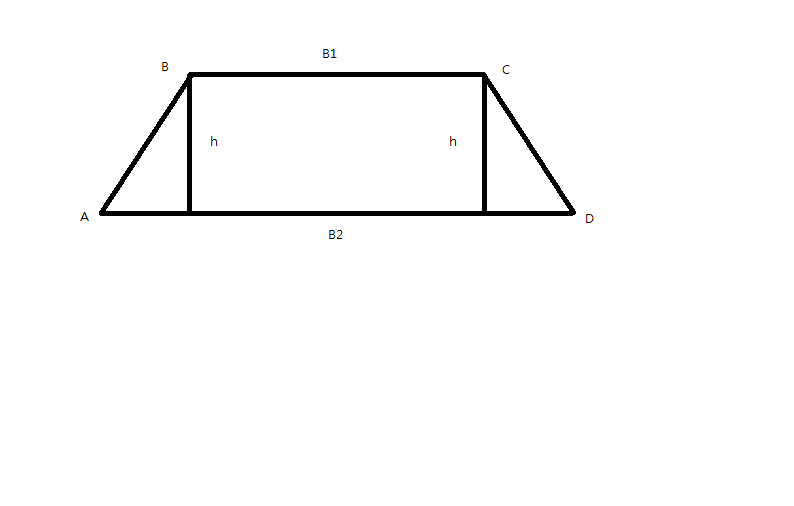
\includegraphics[height=0.7\textheight]{./img/rectangle_in_trapezoid.png}
\end{itemize}
\end{frame}

\begin{frame}
\frametitle{Accelerometer}
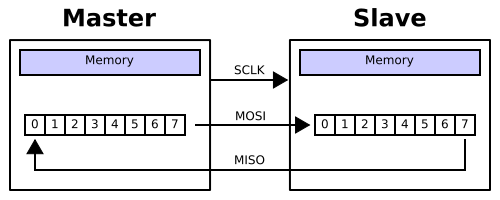
\includegraphics[scale=0.4]{img/spi}
\begin{itemize}
\item SPI digital interface -- FPGA is master, accelerometer slave
\item Accelerometer has different registers for x, y, z acceleration, signal which register to read
\item Configurable SPI clock, but will still need to cross clock domains
\item Accelerometer is noisy -- some sort of low pass filter needed
\item Accelerometer nonlinearities -- lookup table needed?
\end{itemize}
\end{frame}

\begin{frame}
\frametitle{Audio System - Motivation}
\begin{itemize}
	\item Auditory feedback is more effective
	\item Important for frequent setups or adjustments
	\item Highlight important details without affecting UI
\end{itemize}
\end{frame}

\begin{frame}
\frametitle{Audio System - Functionality}
\begin{itemize}
	\item Calibration instructions
	\item Two-Axis Tilt Angle
	\item Percentage of pixels utilized
\end{itemize}
\end{frame}

\begin{frame}
\frametitle{Audio System - Implementation}
\begin{itemize}
	\item Wave files -{software}-> Bit Files -{USB/FTDI}-> Labkit -{labkit_receiver.v}-> CF Card
	\item // ADD in image with data flow
	\item Pre-recorded audio samples on CF Card
\end{itemize}
\end{frame}

\begin{frame}
\frametitle{Audio System - Interface}
\begin{itemize}
	\item // ADD in image with an enlarged version of the module highlighting interface
	\item Set of triggers and data as interface.
\end{itemize}
\end{frame}

\begin{frame}
\frametitle{Responsibilities}
\begin{itemize}
	\item{Ganesh}
	\begin{itemize}
		\item Identifying Tilt Compensation Algorithm, considering:
		\begin{itemize}
			\item Complexity
			\item hardware constraints
			\item implementability
		\end{itemize}
		\item Transform Module
	\end{itemize}
	\item{James}
	\begin{itemize}
		\item Accelerometer
		\begin{itemize}
			\item Interfacing
			\item Noise reduction
		\end{itemize}
		\item Calibration module
	\end{itemize}
	\item{Shantanu}
	\begin{itemize}
		\item Audio output
		\begin{itemize}
			\item Audio Samples
			\item Triggers for each output
		\end{itemize}
		\item Audio module
		\item Test Setup
	\end{itemize}
\end{itemize}
\end{frame}

\begin{frame}
\frametitle{Timeline}
\begin{description}
	\item{Nov. 10}
	\begin{itemize}
		\item Initial module implementation
	\end{itemize}
	\item{Nov. 17}
	\begin{itemize}
		\item Module Integration & module debugging
	\end{itemize}
	\item{Nov. 24}
	\begin{itemize}
		\item System Integration debugging
	\end{itemize}
	\item{Dec. 1}
	\begin{itemize}
		\item Real World Testing & Stretch Goals
	\end{itemize}
\end{description}
\end{frame}

\begin{frame}
\frametitle{References}
\bibliographystyle{plainnat}
\bibliography{references}
\end{frame}

\end{document}
